%%%%%%%%%%%%%%%%%%%% book.tex %%%%%%%%%%%%%%%%%%%%%%%%%%%%%
%
% sample root file for the chapters of your "monograph"
%
% Use this file as a template for your own input.
%
%%%%%%%%%%%%%%%% Springer-Verlag %%%%%%%%%%%%%%%%%%%%%%%%%%


% RECOMMENDED %%%%%%%%%%%%%%%%%%%%%%%%%%%%%%%%%%%%%%%%%%%%%%%%%%%
\documentclass[pdftex,12pt, oneside, a4paper]{book}

% choose options for [] as required from the list
% in the Reference Guide, Sect. 2.2
%\usepackage[paperwidth=8.5in, paperheight=13in]{geometry}

\usepackage{makeidx}         % allows index generation
\usepackage{graphicx}        % standard LaTeX graphics tool
                             % when including figure files
\usepackage[bottom]{footmisc}% places footnotes at page bottom
\usepackage[english]{babel}
\usepackage{enumerate}
\usepackage{paralist}
\usepackage{float}
\usepackage{gensymb}  
\usepackage{listings}
\usepackage{color} 
\usepackage{array}

% make quote in italic
\newenvironment{italicquotes}
  {\begin{quote}\itshape}
  {\end{quote}}
% etc.
% see the list of further useful packages
% in the Reference Guide, Sects. 2.3, 3.1-3.3

% definisi warna untuk kode program
\definecolor{codegreen}{rgb}{0, 0.6, 0}
\definecolor{codegray}{rgb}{0.5, 0.5, 0.5}
\definecolor{codepurple}{rgb}{0.58, 0, 0.82}
\definecolor{backcolor}{rgb}{0.95, 0.95, 0.92}

% list code custom style
\lstdefinestyle{mystyle} {
  backgroundcolor=\color{backcolor}, 
  commentstyle=\color{codegreen},
  keywordstyle=\color{magenta}, 
  numberstyle=\tiny\color{codegray},
  stringstyle=\color{codepurple},
  basicstyle=\footnotesize,
  breakatwhitespace=false, breaklines=true, captionpos=b, keepspaces=true,
  numbers=left, numbersep=5pt, showspaces=false, showstringspaces=false,
  showtabs=false, tabsize=2
}

% mystyle for listing set
\lstset{style=mystyle}

\newcommand{\HRule}{\rule{\linewidth}{0.5mm}}

\makeindex             % used for the subject index
                       % please use the style svind.ist with
                       % your makeindex program


%%%%%%%%%%%%%%%%%%%%%%%%%%%%%%%%%%%%%%%%%%%%%%%%%%%%%%%%%%%%%%%%%%%%%

\begin{document}

\begin{titlepage}

\begin{center}
{\large BUKU PETUNJUK ANALISA SISTEM INFORMASI GEOGRAFIS PBB-P2 DENGAN QUANTUM GEOGRAPHICAL INFORMATION SYSTEM (QGIS)}

\HRule\\[1cm]

PERIODE PENILAIAN TAHUN 2016\\[1cm]


\includegraphics[width=0.5\textwidth]{./resources/logo}\\[1cm]

Oleh :\\
Priyanto Tamami, S.Kom.\\
NIP 19840409 201001 1 025\\
Dinas Pendapatan dan Pengelolaan Keuangan\\
Pemerintah Kabupaten Brebes\\[1cm]

\vfill

Tim Penilai\\
Jabatan Fungsional Pranata Komputer\\
Badan Pusat Statistik\\
Brebes, DD MMMM 2016
\end{center}

\end{titlepage} 

\frontmatter%%%%%%%%%%%%%%%%%%%%%%%%%%%%%%%%%%%%%%%%%%%%%%%%%%%%%%

%\include{dedic}
%\include{pref} 

\begin{center}
{\huge \bfseries Lembar Pengesahan}\\[0.4cm]



\begin{tabular}{l c p{10cm}}
  Nama Kegiatan & : & Membuat Petunjuk Operasional Sistem Komputer \\
  Judul & : & BUKU PETUNJUK ANALISA SISTEM INFORMASI GEOGRAFIS PBB-P2 DENGAN QUANTUM GEOGRAPHICAL INFORMATION SYSTEM (QGIS) \\
\end{tabular}\\[2cm]

\begin{tabular}{c c}
  Disetujui oleh : & Disusun Oleh \\
  Kepala Seksi Pendataan, Penetapan, dan Keberatan & Pranata Komputer \\
  Pada tanggal DD MMMM 2016 & Selesai tanggal : DD MMMM 2016 \\
  & \\
  & \\
  & \\
  Fetiana Dwiningrum, SIP, M.Si. & Priyanto Tamami, S.Kom \\
  NIP 19880223 200701 2 001 & NIP 19840409 201001 1 025
\end{tabular}

\end{center} 

\tableofcontents
\listoffigures

\mainmatter%%%%%%%%%%%%%%%%%%%%%%%%%%%%%%%%%%%%%%%%%%%%%%%%%%%%%%%
\chapter{\textit{DOWNLOAD} DATA OSM}

QGIS walaupun tergolong dalam perangkat lunak terbuka dan gratis, namun menyediakan fasilitas bukan hanya sebagai editor data spasial, tetapi mampu memberikan beberapa fasilitas analisis, baik terhadap data spasial, maupun data atribut.

Pada Bab ini akan dibahas bagaimana cara memperoleh data spasial dalam format vektor dari \textit{Open Street Map} menggunakan \textit{Tools} yang ada pada QGIS yang mungkin dapat dijadikan salah satu sumber data dalam analisa.

Untuk melakukan pengambilan data dari OSM, QGIS memerlukan 2 (dua) \textit{plugins}, adapun tahapan-tahapan yang dapat dilakukan sebagai berikut :

\begin{enumerate}[1.]
  \item Meng\textit{install plugin} \textbf{OSMDownloader} dan \textbf{OpenLayers} melalui menu \texttt{Plugins > Manage and Install Plugins...} seperti pada gambar \ref{fig:managepluginsmenu}.
  
  \begin{figure}[H]
    \centering
    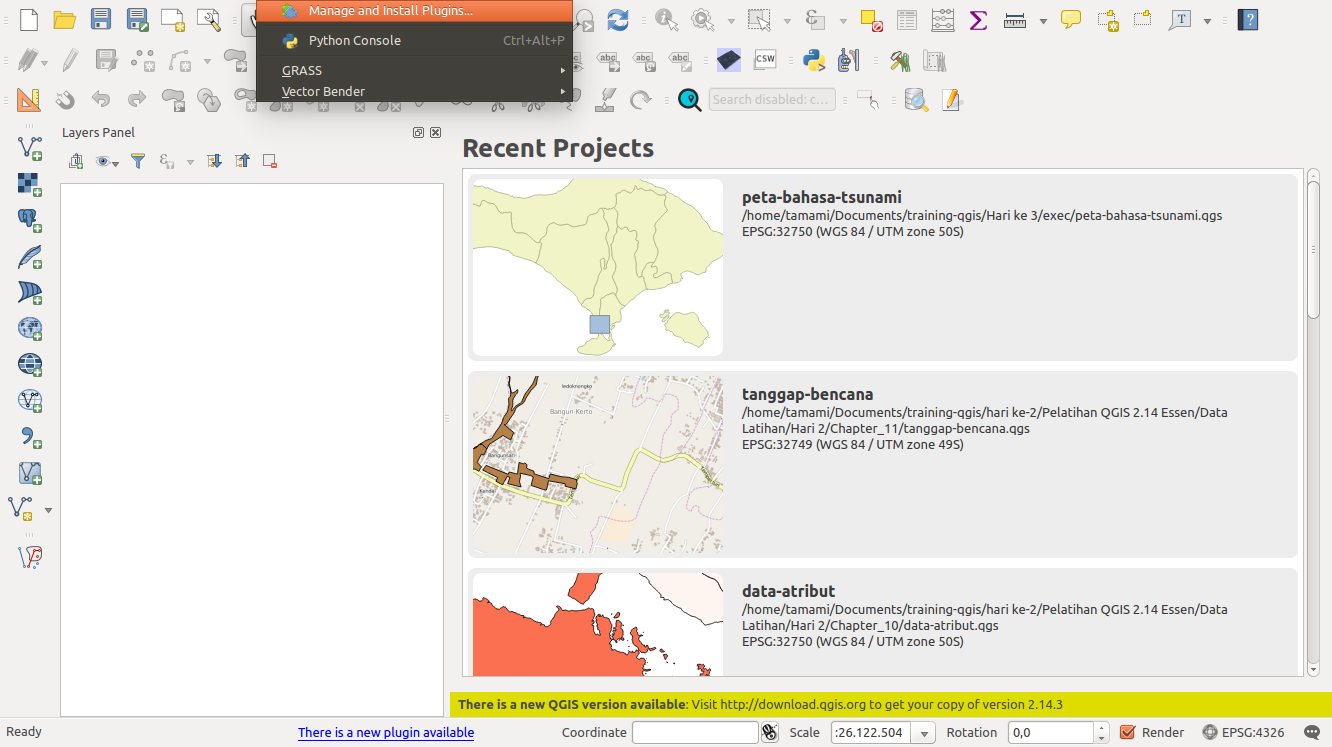
\includegraphics[width=1\textwidth]{./resources/001-manage-plugins-menu}
    \caption{Menu \textit{Manage Plugins}}
    \label{fig:managepluginsmenu}
  \end{figure}
  
  \item Kemudian ketik kata kunci \texttt{OSM} di bagian \textit{search} pada kotak dialog dibagian atas dan pilih komponen seperti pada gambar \ref{fig:osminstallwin}
  
  \begin{figure}[H]
    \centering
    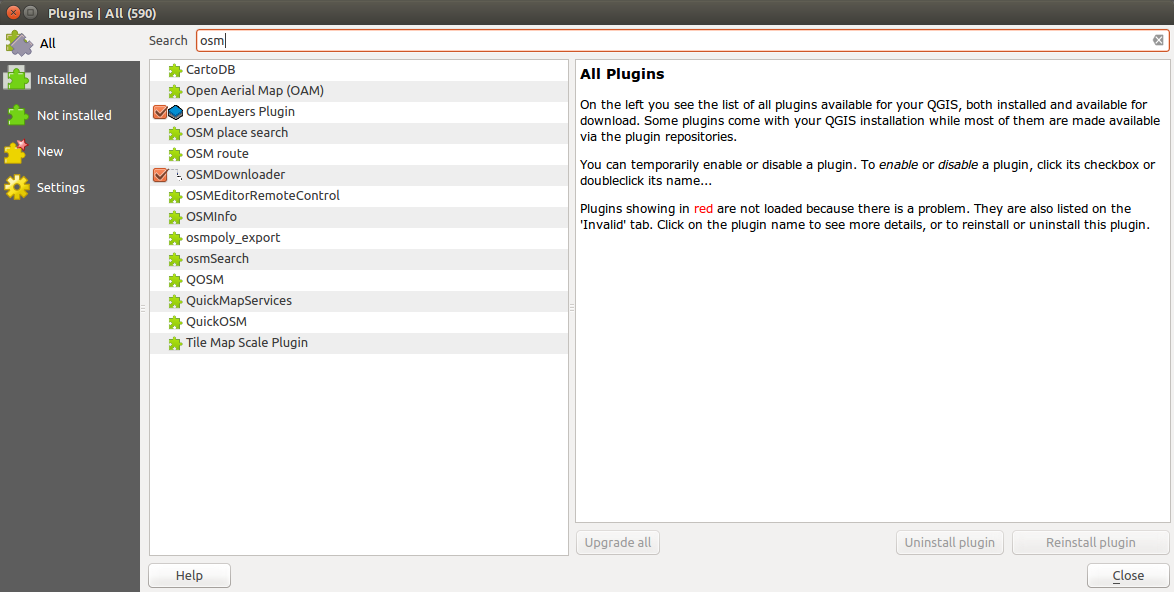
\includegraphics[width=1\textwidth]{./resources/002-osm-install-win}
    \caption{Jendela \textit{Manage Plugins}}
    \label{fig:osminstallwin}
  \end{figure}
\end{enumerate}
%\include{04.data-sig}
%\include{05.instalasi-qgis} 
%\include{06.pengenalan-ui} 
%\include{07.sistem-referensi-koordinat} 
%\include{08.georeferensi-data-raster} 
%\include{09.membuat-data-spasial}

\backmatter%%%%%%%%%%%%%%%%%%%%%%%%%%%%%%%%%%%%%%%%%%%%%%%%%%%%%%%
\printindex

%%%%%%%%%%%%%%%%%%%%%%%%%%%%%%%%%%%%%%%%%%%%%%%%%%%%%%%%%%%%%%%%%%%%%%

\end{document}